\documentclass{beamer}
\usetheme{JuanLesPins}
\usecolortheme{default}
\usepackage{graphicx}
\usepackage[utf8]{inputenc}
\usepackage[T1]{fontenc}
\usepackage[scriptsize]{caption}
\title{Parallel Gaussian Elimination}
\author{Szymon Maj \& Jarosław Szczęśniak}
\institute{Akademia Górniczo-Hutnicza im. Stanisława Staszica w Krakowie}
\begin{document}

	\begin{frame}
		\titlepage
	\end{frame}

	\section{Wstęp}
	\begin{frame}
		Jedna z najszybszych metod, doprowadzająca do dokładnego rozwiązania przez wykonanie skończonej ilości działań.
		\newline \\
		Pozwala na:
		\begin{itemize}
			\item rozwiązanie układó równań liniowych,
			\item obliczanie rzędu macierzy,
			\item obliczanie macierzy odwrotnej.
		\end{itemize}
	\end{frame}
	
	\section{Historia}
	\begin{frame}
		\begin{columns}
		\column{3in}
			Nazwa metody pochodzi od nazwiska niemieckiego matematyka Carla Friedricha Gaussa, żyjącego na przełomie XVIII i XIX wieku.
			\newline \\
			Doszukano się podobieństw w ,,The Nine Chapters on the Mathematical Art’’, chińskich zapiskach matematycznych, które powstawały między X wiekiem p.n.e. a I wiekiem n.e.
		\column{1.5in}
			\begin{figure}
				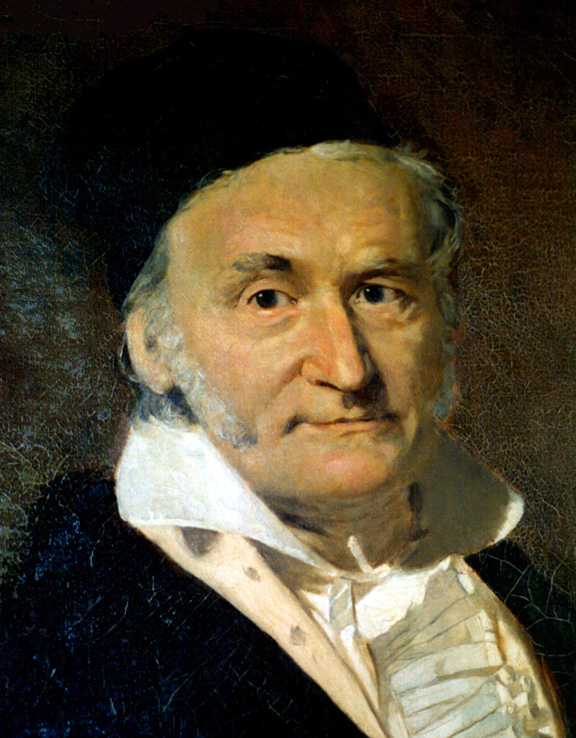
\includegraphics[scale=0.3]{gfx/Carl_Friedrich_Gauss.jpg}
%				\caption{ Strona z ,,The Nine Chapters on the Mathematical Art’’ }
			\end{figure}
			\begin{figure}
				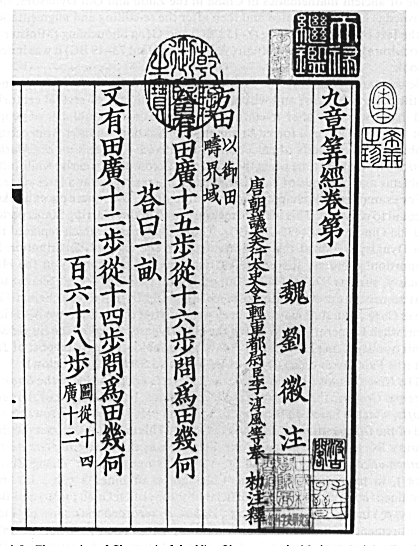
\includegraphics[scale=0.2]{gfx/tncotma.png}
%				\caption{ Strona z ,,The Nine Chapters on the Mathematical Art’’ }
			\end{figure}
		\end{columns}		
	\end{frame}
	
	\section{Algorytm}
	\begin{frame}
		Metoda składa się z dwóch części:
		\begin{enumerate}
			\item Eliminacja w przód
				\begin{itemize}
					\item wynikiem jest macierz trójkątna
					\item usuwanie niewiadomych z kolejnych wierszy macierzy
					\item operacje elementarne - dodawanie, mnożenie, zamianę wierszy
				\end{itemize}
			\item Podstawianie wstecz
				\begin{itemize}
					\item warunek - macierz trójkątna
					\item obliczenie wartości zmiennych od dołu macierzy
					\item podstawianie wartości obliczonych zmiennych w poprzednich równaniach, dochodząc do początku
				\end{itemize}
		\end{enumerate}
		Złożonośc obliczeniowa metody wynosi O($n^3$).
	\end{frame}
	
	\section{Algorytm równoległy}
	\begin{frame}
		\begin{itemize}
			\item Dekompozycja na poziomie wierszy
			\item W każdym kolejnym kroku jeden z wierszy (pivot), odejmujemy z odpowiednim współczynnikiem od każdego następnego wiersza
			\item Operacja odejmowania w tym przypadku jest niezależna, więc można ją zrównoleglić
			\item Odejmowany wiersz (pivot) zmieniany jest po zakończeniu pracy wszystkich procesorów
			\item Z każdym kolejnym krokiem ilość operacji zmniejsza się
			\item Problemem jest narzut komunikacji
		\end{itemize}
	\end{frame}

	\section{Bibliografia}
		\begin{frame}
		\frametitle{Bibliografia}
			\begin{thebibliography}{1}
				\bibitem{pge}{S.F.McGinn and R.E.Shaw - ,,Parallel Gaussian Elimination Using OpenMP and MPI’’ - University of New Brunswick}
			\end{thebibliography}
		\end{frame}
		
\end{document}